\section{Introduction}
\label{sec:intro}

Since the introduction in 2015, Ethereum has gained much interest from projects and companies to launch their decentralized applications on the network. As a result, Ethereum network has suffered from several congestions in the past due to, for example, popular token sales or games like Cryptokitties. In such occasions, users either have to pay much higher fees to send their transactions, or have to wait for hours to get their transactions confirmed. To date, Bitcoin’s peak is around $425,000$ transactions per day~\footnote{\url{https://blockchain.info/charts/n-transactions?timespan=all}} and Ethereum's is $1.4$ million~\footnote{\url{https://etherscan.io/chart/tx}}, both are way behind $150$ million daily active users on Twitter, and much smaller compared to $1.4$ billion users on Facebook. In addition, the average block latency of 15 seconds on Ethereum poses more challenges in building an usable platform for most users. Both scalability and latency constraints make it harder for decentralized applications to be mainstream.

Let's use decentralized exchanges as an example, existing decentralized exchanges suffer from major problems, including, but not limited to, low liquidity, poor user experience, poor scalability (due to the underlying infrastructure). While there are different proposals to tackle these challenges, each solution makes significant compromise in either security, decentralization or supporting features. For example, our current KyberNetwork exchange allows optimal security by running entirely on-chain, allowing better user experience with a few simple clicks to finish a trade, but is not able to support limit orders, trading leverage, or high frequency trading yet. Other exchanges like 0x~\footnote{\url{https://0xproject.com/}} and EtherDelta~\footnote{\url{https://etherdelta.com/}} attempt to simulate trading experience on centralised exchanges by employing a hybrid model, i.e. having an off-chain (centralized) orderbook and doing on-chain settlement. There is a clear security tradeoff since users essentially have to rely on the server/website that stores and provides the orderbook. Regardless, all these solutions suffer from scalability constraint and long latency settlement since each settlement incurs one on-chain transaction on the Ethereum blockchain. At the time of writing, the latency is around 15 seconds on average and the Ethereum blockchain can process around 10-15 transactions per second depending on the transaction types. Further, users may have to pay much higher transaction fees to pay for the transaction gas when the blockchain is busy with events like Cryptokitties or some high profile public token sales. Clearly, such solutions are not able to compete with centralized exchanges like Binance~\footnote{\url{https://www.binance.com/}}, Huobi~\footnote{\url{https://www.huobi.pro/}} and the likes. In the current report~\cite{binance-report}, Binance claimed to process $40,000$ requests per second at its peak, leaving all decentralized exchanges performance far behind. If there are no significant design changes, decentralized exchanges are only usable by a few, and won't be able to attract mainstream users, not to mention professional traders.

Recently, Plasma arrived to the rescue with promising scalability by pushing transactions to a separate blockchain and using crypto-economic to protect user from malicious blockchain validators~\cite{plasma}. However, the existing Plasma design is meant to be high level and not optimized for decentralized exchanges. The scaling of Plasma is also bounded by the physical capacity of the Plasma validators, hence it does not offer optimal scaling without compromising user experience and security guarantee~\footnote{To be precise, the Plasma whitepaper mentions the concept of Plasma child chain. Technically it works and offers infinite scalability, but with the cost of user experience since they have to move their assets to many layers. Not to mention that the Plasma child chain is another layer of tradeoff for security guarantee.}. If we use the scale of Binance to measure, each Plasma node may have to store Terabytes of data and network bandwidth, which may require infrastructure of a medium to large server to operate. Regardless, there has not been discussion regarding interoperability, and censorship resistance when it comes to Plasma.


Scalability apparently is the problem for not only DEXes, but also for many other applications including social networks, games. For example, Etheremon~\footnote{\url{https://etheremon.com}} and Peepeth~\footnote{\url{https://peepeth.com}} are currently employing a tradeoff that does batch commitment of activities on-chain to offer better usability. The activities that are not yet committed are stored locally within the project servers, that tremendously reduces the security of the system.

In this paper, we introduce \codename, a novel protocol design for secure and scalable blockchain with low latency. At a high level, \codename finds the sweet spot between both Plasma and sharding to i) allow transactions to happen on a sidechain securely with much lower block time; and ii) enable linear scaling without requiring more resources from nodes or validators in the network. The tradeoff is that \codename is not a generic design --- it works well for only a class of applications that have different components and these components seldom interact with each other. For example, in the case of decentralized exchange, one can consider each trading pair as one component of the exchange, and there are much less interactions between different trading pairs than within a trading pair. Thus, we can efficiently apply sharding for decentralized exchanges to spread the workload to different shards and achieve much higher scalability.
In addition, \codename also takes into account interoperability in its design, i.e. moving assets like Bitcoin, Litecoin, ETC or any cryptocurrency from a different blockchain to the Plasma chain. Similarly, \codename can be applied for applications like Etheremon and Peepeth to offer better security guarantee without sacrificing user experience.

For ease of understanding, in the later sections, we describe \codename in the context of decentralized exchanges in this paper and mention how to apply it to other applications in Section~\ref{sec:others}.

\subsection{Desired properties}
Given the state of the art of decentralized exchanges and the feedback from users to Kyber Network after a few months of deployment, we describe the desired properties for a high performance decentralized exchange (DEX) as follows.

\begin{itemize}
\item \textbf{Scalability}. The DEX should be able to allow millions of users trading everyday, processing billions of trades without requiring significant hardware and network bandwidth from validators (or nodes) in the DEX. Further, it may happen that a few popular trading pairs may occupy all capacity of the DEX, hence affecting the trading experience of users on other pairs. A scalable DEX should prevent such problems and allow users to trade all user pairs smoothly.
\item \textbf{Low latency}. The DEX should allow low latency trading, i.e. the time between when an order is submitted and when it is confirmed should be of a few seconds, if not milliseconds. We aim to achieve 2-second confirmation and instant settlement in our design.

\item \textbf{Security and decentralization}. This is the fundamental property for a DEX and the reason why people prefer a DEX over centralised exchanges. Decentralization matters more in DEXes since there is a great demand for better transparency and censorship-resistant in exchanges. Recently there have been questions regarding how transparent the centralized exchanges operate~\footnote{\url{https://medium.com/@sylvainartplayribes/chasing-fake-volume-a-crypto-plague-ea1a3c1e0b5e},\newline \url{https://cointelegraph.com/news/okex-resolves-futures-price-slip-impact-as-trader-threatens-suicide}}

\item \textbf{Interoperability}. The DEX should allow people to trade different cryptocurrencies, including but not limited to Bitcoin, Ethereum, Litecoin, Ethereum Classic, EOS, and so on. This should be done without any compromise of other properties.
\end{itemize}
These are the main desired properties that a DEX must have in order to be able to compete with centralized exchanges. There are non-protocol ideal properties that are also important when it comes to deployment and adoption including high liquidity, good user experience, etc. However, these properties are orthogonal to the main problem of building a high performance decentralized exchange that we are building.

\section{Related work}
\textbf{Why not having a tree of plasma chains?} A careful reader may wonder what is the difference between \codename and a tree of Plasma chains, i.e. having separate child plasma chain on top of the existing plasma chain. The reason is that Plasma is a layer-2 solution, i.e. it creates a separate layer on top of the root-chain. In general layer-2 solutions have specific security trade-offs, for example in Plasma users have to watch the validator to see if something bad happens and exit before it is too late. Having more ``layer-2” solutions on-top of a Plasma chain will introduce more security trade-offs and makes it much harder for users to follow. It is also harder for developer to either build the platform or even reason about the security guarantee of the platform. On the other hand, sharding offers scalability at the consensus layer, without any compromise in security. The major trade-off when it comes to sharding is usability due to cross-shard transactions. However, in \codename we have a clear logic of separating the network into different shards for different trading pairs, minimizing the amount of cross-shard transactions.

\textbf{How about existing sharding chains like Zilliqa?} One may wonder why we do not build a platform on top of Zilliqa, as Zilliqa is already building a scalable blockchain using sharding. The main difference is that Zilliqa does not support state sharding, and is not optimised for a decentralized exchange platform or any other application. Requirements from storage and state updates when processing billions of transactions will cost validators in Zilliqa more storage, bandwidth, and computation resources. On the other hand, \codename offers a clear separation of state processing, trading activities and storage. We also leverage Plasma to allow a smaller set of validators in shard, hence supporting lower latency for our trading platform.

\textbf{Atomic Cross-Chain Swap (ACCS).}~\cite{atomic-swap-wiki} is one of the earliest and simplistic design based on contracts with nLockTime whose payout is redeemable through revealing a preimage of a previously committed hash (a formal description could be found in Section 2 of Tesseract~\cite{tesseract}). The main problems with ACCS are threefold: high latency introduced by timelock which makes real-time exchange impossible, this is problem is fundamentally a result of \textit{fair exchange problem}\cite{fair-exchange-impossibility}; poor scalability due to complexity in the context of multi-party ACCS with interleaving expiring timelocks; and slow order discovery and limited liquidity. In comparison, \codename tokenizes other cryptocurrencies, thus significantly reduce the intricate approach towards interoperability. It is worth noting that \codename does not solve long latency in cross chain transfer by itself. However once pegged tokens are minted, they could be easily traded like any other tokens and be considered as confirmed once finalized on \codename.

\textbf{Payment and State Channels.}\cite{lightning, miller2017sprites} are constructions that offloads transactions from Blockchain via locked state deposits and eventually settle on-chain with updated states. Particularly, the recently published \textit{generalized state channel} utilizes counterfactually instantiated contracts for installing new functionalities without broadcasting to the blockchain~\cite{Coleman2018, Dziembowski2018}. While they scale blockchain throughput efficiently, they are ill-suited for applications like DEX as states are kept only known to direct participants within a channel, which leaves a global order book almost impossible to be built.

\section{Design}

Most of our design leverages existing work in Plasma~\cite{plasma} and our previous work in sharding~\cite{elastico}, blockchain interoperability~\cite{peacerelay}. Our goal is to achieve all the aforementioned desired properties with the least compromise in security and decentralization.

\begin{figure}[t]
  \centering
  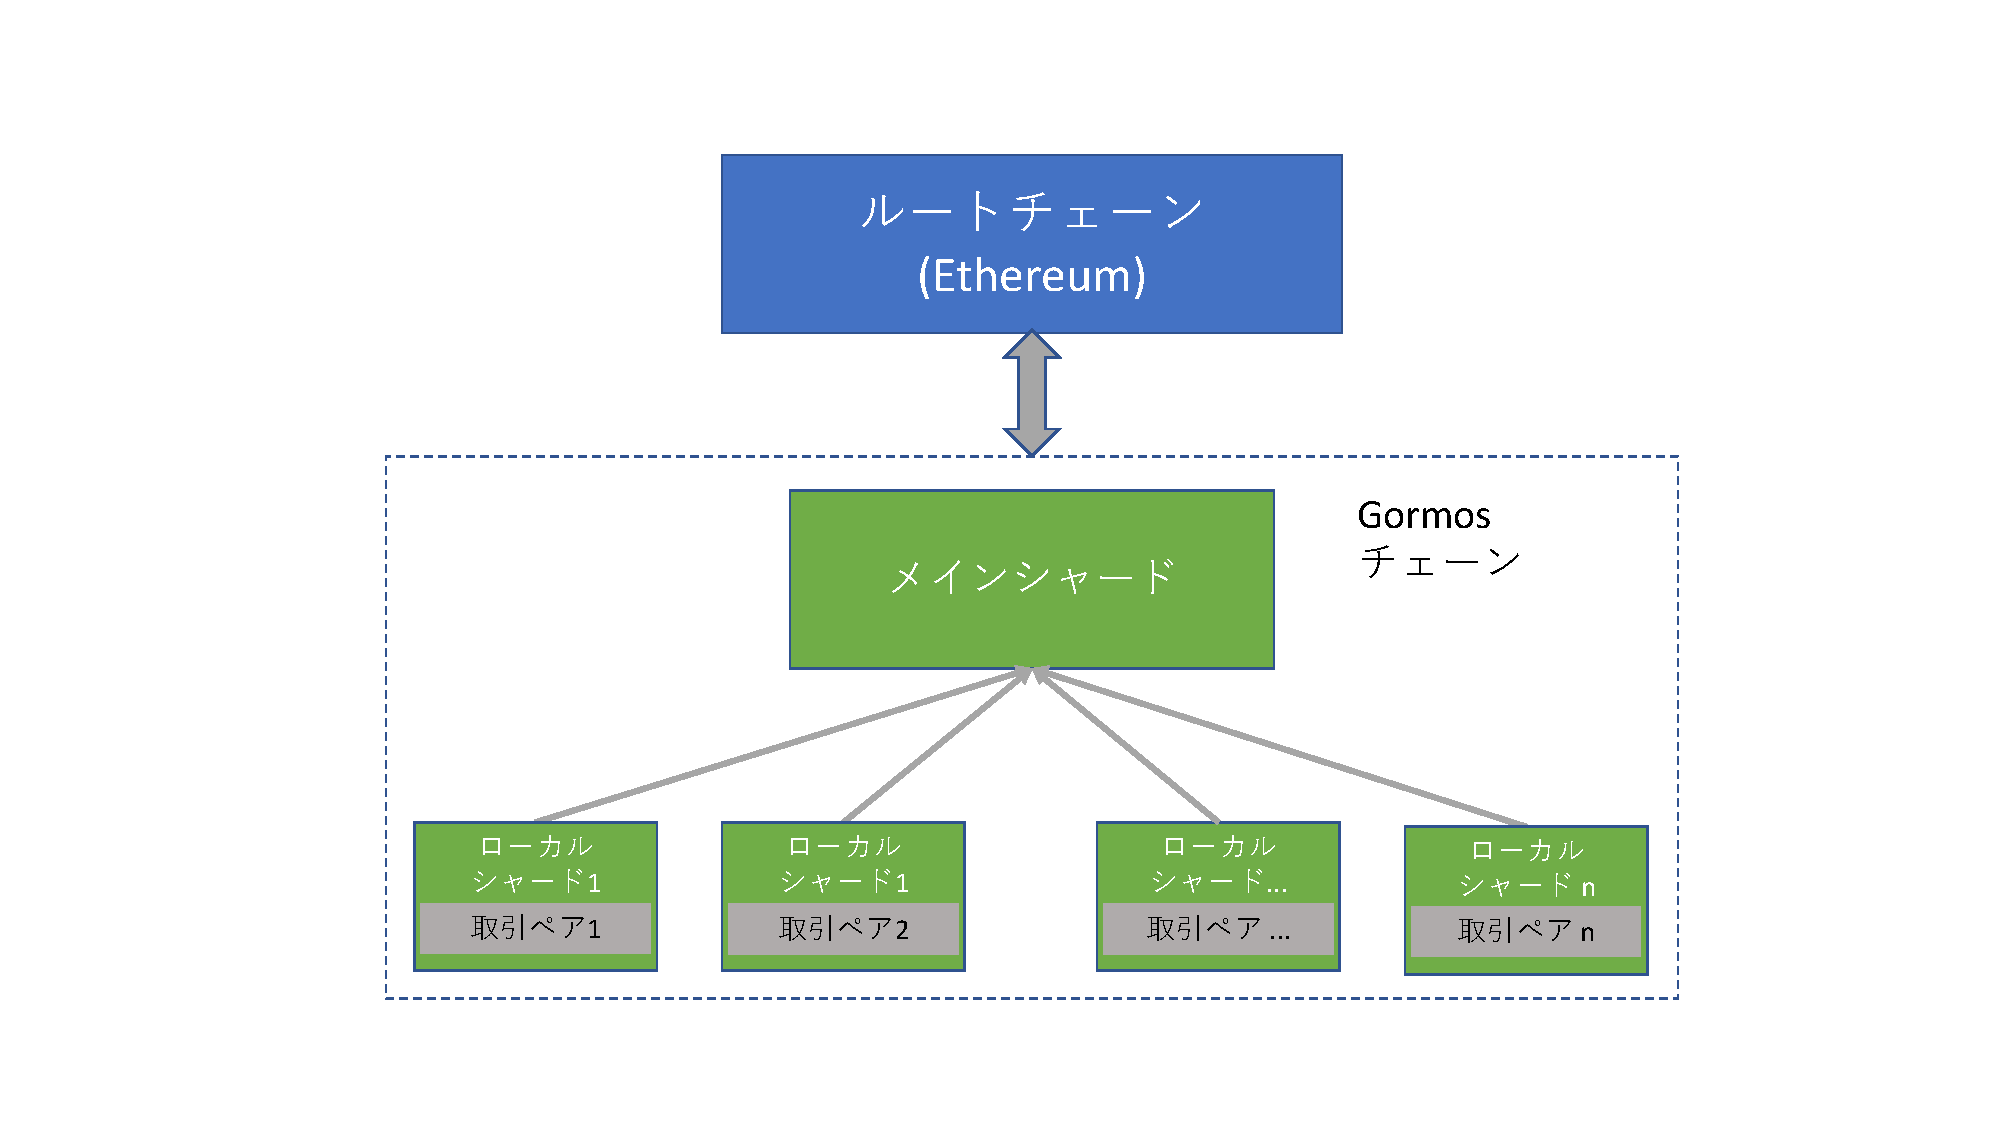
\includegraphics[width=0.8\textwidth]{images//architecture}
  \caption{\codename System Architecture}
  \label{architecture}
\end{figure}


\subsection{Design Overview}
The high level of \codename's design is shown in the Fig.\ref{architecture}. \codename employs both prominent technologies namely plasma and sharding. This Plasma-based approach with built-in sharding architecture allows listing infinite trading pairs without adding scaling pressure\footnote{More accurately, asymptotically optimal (i.e. constant factor cost) in main shard with increasing token pairs/shard, linear scaling within shard with increasing computations and communication costs incurred by more users.} to the existing trading platform.

We realized that building a high performance DEX on-top of existing public blockchains is hard, as the infrastructure is not yet ready. In order to allow a better latency and more scalability without sacrificing security, we employ Plasma model in which there is a separate blockchain which is periodically committed its state back to the root chain (i.e. Ethereum chain). We employ a Byzantine Agreement within the validators of the new chain to achieve low latency and faster finality. More importantly, we also design a sharding architecture on top of this Plasma chain to allow infinite scaling. Our observation is that activities of different trading pairs can be clearly separated and localized in different shards. For example, trades between ETH/KNC and BTC/OMG can be separated and users who trades between ETH/KNC should not affect users who trade BTC/OMG. With this design, we can add more shards should the platform list more tokens, without affecting the performance and trading experience of the existing listing pairs. Such a design can scale up to a large number of trading pairs, and support millions of trades per second, yet require least amount of resources from validators. Validators in \codename do not have to store the entire states nor process every trade happening in the platform. Instead, they only have to store the state for their shards and process all trades for the corresponding trading pairs listed in their shard. Adding more trading pairs does not affect validators in existing shards.

\textbf{Rationale of \codename design.} At its core, \codename combine both sharding and Plasma approaches and use one's advantage mitigating the limitations of the other. Specifically, \codename leverages Plasma to reduce latency of sharding, and employs sharding to scale up Plasma even further. \codename does so through making a tradeoff on the generality or the universal applicability of this design. That means \codename is application specific and only works best with a particular class of decentralized applications with clear separation among their sub-components.


Putting the core observations described earlier all together, a heuristic rationale of \codename could now be established. A more detailed comparison between sharding, Plasma and \codename is shown in Table \ref{comparison}.

\begin{table}
  \centering
  \begin{tabular}{|C{1.5cm}|C{2.2cm}|C{1.5cm}|C{3.2cm}|}
    \hline
    & \textbf{Scalability} & \textbf{Latency} &\textbf{Applicability} \\
    \hline
    \textbf{Plasma} & 100x & Low & Generic \\
    \hline
    \textbf{Sharding} & 100x & High\footnote{for standalone blockchain with sharding} & Somewhat Generic\\
    \hline
    \textbf{\codename} & \textbf{1000x\xspace-\xspace10000x} & \textbf{Low} & \textbf{Application Specific} \\
    \hline
  \end{tabular}
  \vspace{2pt}
  \caption{Plasma vs. Sharding vs. \codename}
  \label{comparison}
  \vspace{-20pt}
\end{table}


\subsection{Plasma: move trading activities to a new sidechain securely}
At high level, Plasma offers a security-performance tradeoff by having a sidechain with cryptoeconomic incentives to prevent malicious validators from cheating users. Users in Plasma chain can move their assets from the root-chain (i.e. Ethereum chain) to the Plasma chain, and still transact and operate in this Plasma chain safely, without having to make transactions in the root chain. If anything happens, e.g. the validators in the Plasma chain equivocate or do not credit the right balance for users, users can submit a ``fraud proof" to the root chain to “exit” and get their assets back. Thanks to this design, more transactions are processed ``off the root chain" yet users can still get good security guarantee.

One advantage in Plasma is that the validator set can be small without affecting the security guarantee, i.e. Plasma chain can even work with one single validator. Thus, the performance of a Plasma chain can be as good as a centralized server. However, due to the need for decentralization to offer better fault tolerant and censorship resistance, one must have more validators in the validator set. Given this trade off, and to achieve fast settlement, we may decide to go with a validator set of size of around $20$. We explain more on the choice of the validator set in the Section~\ref{sec:details}.

\subsection{Sharding to offer optimal horizontal scalability}
As aforementioned, the goal of our sharding solution is to separate different trading tokens to different shards, e.g. a few token pairs per shard. The high level idea in sharding is to distribute the validators to different subsets (or shards), each subset of validators maintains, or is responsible for a separate portion of activities in the Plasma chain. Previous work has proposed several generic sharding protocols~\cite{elastico, omniledger, zilliqa}, however no previous work has proposed a specific design that works best for decentralized exchanges.

In \codename, we use the 2-layer architecture in our design: there is a main shard and there are several local shards. The local shards take care of trading for a few specific token pairs while the main shard collects and aggregates the results from local shards. The base currencies (ETH, BTC) can exist in the main shard and local shards, while the other tokens only exist in one designated shard. This approach makes sense since trading between different pairs are not related, hence no need to store and process every trade in one single chain. This is inspired by sharding in centralized exchanges, i.e. most centralized exchanges already handle different trading pairs in different servers. This design not only provides a scalable architecture but also offers a clear separation of risks. For example, if a token is not functional for some reason (i.e. a bug in their token contract like the recent incidents), this shard can pause its trading but other shards can still function as usual.

If a user deposits token from the root chain, the corresponding local shard update the corresponding token’s balance. If user deposit base currencies, the main shard will take care of it. If the user wishes to move the base currencies (ETH, Bitcoin) to a different local shard, the user has to send a transaction to move the coin  from the main shard to the local shard. This design reduces the complexity of cross-shard communication. Specifically, cross-shard communication is only needed when the user wishes to move their base currency, e.g. ETH, from a local shard $i$ to a different local shard $j$. This will require two different transactions, i.e. one to move ETH from local shard $i$ to the main shard, and from the main shard to the local shard $j$.

\begin{figure}[t]
  \centering
  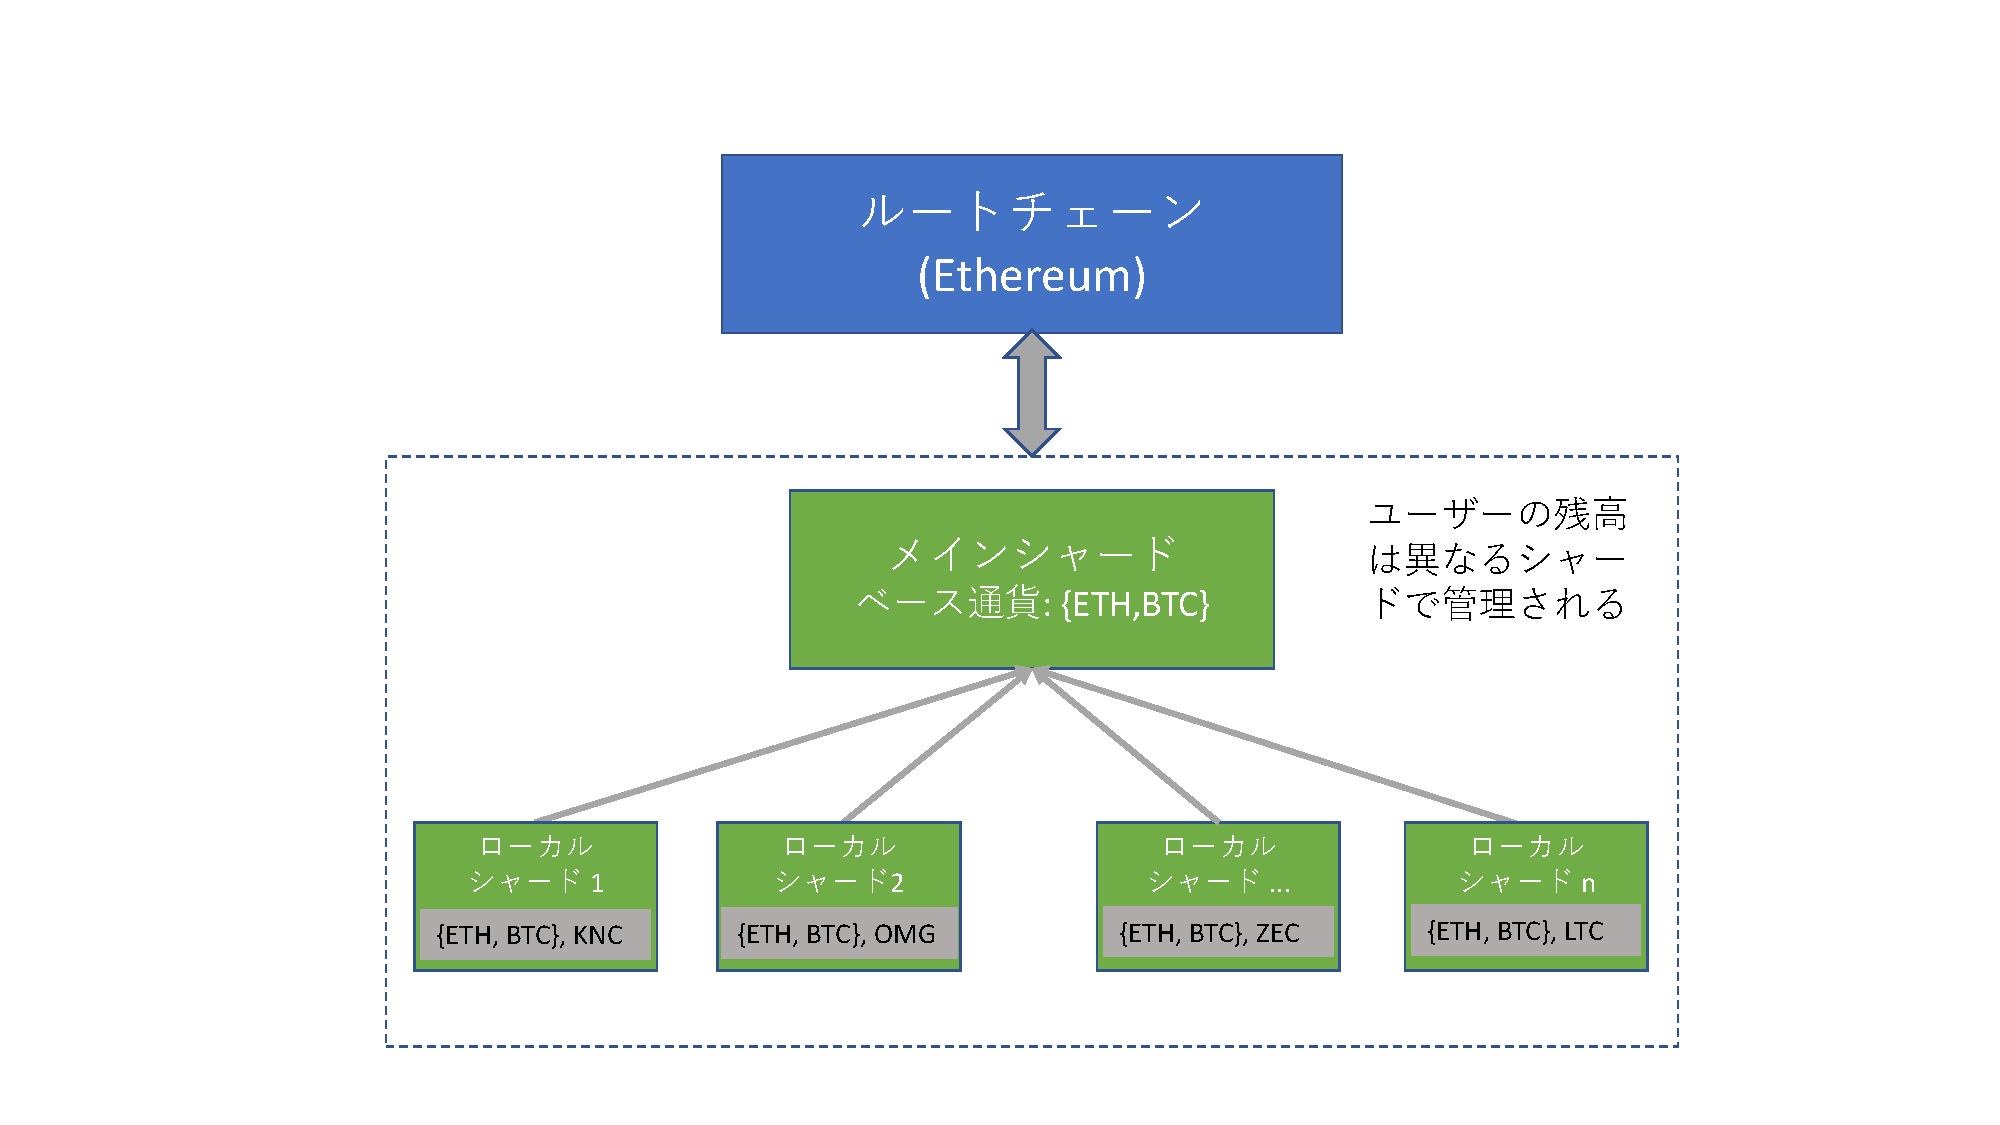
\includegraphics[width=0.8\textwidth]{images//architecture2}
  \caption{\codename's design architecture}
  \label{architecture2}
\end{figure}


The validators within a shard will run a fault tolerant consensus protocol to periodically agree on the latest trades for the token pair the shard. Specifically, after every epoch of 4-5 seconds, the shard validators will issue a new data block that contains the new transactions that represent users’ trade orders since the previous block. A trade order can be a new sell/ buy order, or even a cancellation of some existing order. Based on all the trade requests recorded in a shard, validators can maintain a full orderbook for this token pair in the shard. Validators can also see which trade orders are matched and do the settlement to update the balances of users. The figure below shows an example of a block data and the changes in the balances of users after the block is created. We discuss the details of the trade order format, block structure in a shard in Section~\ref{sec:details}.

\subsection{Shard inspectors: Guardians of the chain}

A good property that makes public blockchains much more attractive than centralized systems is that everything is publicly auditable and verifiable. Thanks to the public key cryptography, every bad or malicious activity can be used to hold the bad actor accountable, i.e. the bad actors can’t deny that they did not do anything wrong given the cryptographic proof. As such, anyone, at anytime, can observe the data from the public blockchain to detect if some wrongdoing is happening, and then identify the malicious actors.
In Plasma, one concern is that users have to be online to observe the Plasma chain and detect if there is wrongdoing done by validators. If so, the users can “exit” by submitting the fraud proof to claim their asset back and penalize the validators. However, our observation is that this action can be done by anyone as the data is publicly available. Third party observers can “exit” on behalf of others. Leveraging this feature, we introduce a new role/ player in every shard which we call shard inspector. Their responsibilities are as below.

Shard inspectors do not participate in the local consensus of the shard, they rather only observe the shards and see if weird things happen to file the report with ``fraud proofs" on main chain and penalize the shard validators.
Shard inspectors also guarantee data availability. They will store all data blocks produced within a shard and can serve data to users. This will guarantee better data availability within a shard.
One can think of shard inspectors as full nodes in Ethereum and Bitcoin, except that these full nodes can ``penalize" the ``miners" (i.e. validators in Plasma chain) by reporting to a higher “authority”. We will discuss in section below the details on how to practically implement this role in \codename, and how to incentivize the inspectors to participate.

\subsection{Interoperability: bridging the many blockchains}

One major problem with existing decentralized exchanges is the ability to support different coins and cryptocurrencies. For example, currently users cannot trade between Bitcoin and other ERC20 tokens on existing decentralized exchanges, due to the fact that there is no seamless solution to move Bitcoin to Ethereum yet. We discuss a few solutions and approaches that \codename considers using to support trading different cryptocurrencies outside of Ethereum ecosystem.
\begin{itemize}

\item PeaceRelay: was an approach that allows users to move EVM-based currencies back and forth the Ethereum main chain. PeaceRelay builds a bi-directional relay between the two chains, and allowing users to “lock” the native coin on one chain to mint a new token that represents the coin on Ethereum in a trustless way. Similarly, users can also burn the said token on Ethereum to “redeem” the coin on the other chain. Apparently one can use PeaceRelay to move Bitcoin from Rootstock to Ethereum and back.

\item Trustless Custodian approach: This recently proposed solution~\footnote{\url{https://blog.kyber.network/bringing-bitcoin-to-ethereum-7bf29db88b9a}} makes it simple for users to generate their Bitcoin token. There is a custodian (not necessarily trusted) who has a public wallet for people to deposit their Bitcoin. The custodian, however, has to collateralize ETH and/ or any other token on Ethereum so that if he acts maliciously, users can report and penalize the validator to claim their Bitcoin back.

\item MakerDao’s approach: MakerDao designs a solution that builds a decentralized stable coin (e.g. DAI) which has its value pegged to 1 USD. Users can collateralize their ETH to mint DAI, and the collateralized asset is always more than the total circulation of DAI. MakerDao relies on the price feed of ETH to value the total collateralized assets. Using the same mechanism, we can using ETH as collateral to mint Bitcoin token, and relying on the ETH:Bitcoin price feed.
\end{itemize}

\subsection{\codename: high performance decentralized exchange}

Based on these core technical components, we build \codename as a high performance decentralized exchange. We show how \codename archive all ideal properties as following.
\begin{itemize}
\item Scalable. \codename embodies two scaling solution in its design, namely Plasma and sharding. While Plasma allows transactions to happen off the root chain with high throughput and cheap (even 0) transaction fees, sharding allows \codename to scale up by separating activities of different trading pairs.
\item Low Latency. An order can be confirmed as soon as a new block in \codename is created, which can be within 4-5 seconds or less depending on the shard configuration. Though we note that it may take longer for the trade to be finalized, i.e. committed back to the root chain.
\item Secure \& Decentralized. \codename allows users to do exit the sidechain and withdraw their assets back to the root-chain if validators do any malicious activities. Further, users can also submit a fraud proof to report and penalize the malicious validators, hence disincentivizing the validators from committing dishonest behaviors. In addition, the consensus within every shard is run by multiple validators, and the validators are frequently rotated among the shards, hence its hard to either compromise a shard or conducting censorship on a particular shard.
\item Interoperability. With various approaches to move Bitcoin and other cryptocurrencies to Ethereum, users can trade different currency pairs on \codename.
\end{itemize}

One good property in our sharding architecture is the clear separation of trading assets. As a result, we can have dedicated shards for different trading asset pairs. One can foresee that \codename will have specific shards that allow people to trade non-fungible tokens. One can also setup a different shard that runs by institutions to facilitate trading of security tokens with different requirements on the user on-boarding. For example, users may need to register and do KYC check in order to do trading on the shard that is supporting security tokens since its dictated by the institutional validators. \codename’s sharding design allows such dynamic yet clear separation of trading activities, thus supporting different ecosystems to co-exist in the same platform.

\section{Technical Details}
\label{sec:details}

We discuss the main technical concerns in this section, starting with how validators are selected, how shards are formed, shuffled and the details on how trades happen in \codename.
% Before we go into the details, we discuss the assumptions that we make in \codename, and explain how to enforce these assumptions in practice.
% Synchronous network for liveness.
% Verifiable Random Function~\ciAlgorand, RandHound]. One can even use the block hash of the root chain for the source of randomness as the random number is not critical in \codename.
% Security of Rootchain (i.e. Ethereum).

\subsection{Validator registration}
In order to be a validator in \codename, users have to deposit KNC on the root chain (Ethereum) as stake. After the deposit is recognized on the Plasma chain, the validator is “registered” and can start the validation process. There are several ways to determine the amount of deposit for validators. One approach is to fix the amount, and accept as many validators as possible. As a result we may have tens of thousands of validators in \codename. Another approach is to leave it to open market and allow only a fixed number (e.g. 1,000), of active validators. One has to put more deposit than the lowest deposit in the current active validator list in order to be a new active validator. The validator with the lowest deposit amount will become inactive after, say, 24 hours. The dynamic deposit allows the market to freely decide how much the validator slot is worth (the main cost for validator is opportunity cost) and how confident they are with the platform.

\subsection{Shard formation}
From the list of active validators, \codename distributes the validators into various subsets, each is responsible for a shard. W.l.o.g, let $N$ be the number of validators, and let $n$ be the number of shards, and each shard will have $c$ validators (so $N = n*c$). If we have more shards ($n$ increases), we can accept more active validators (increase $N$) and support different trading pairs in the newly created shards. Ideally we want to have a uniform distribution in which we rely on a global random number generator with no bias, which can be implemented by VRF~\cite{algorand}, RandHound~\cite{randhound}. However, since the most damage that malicious validators can do is to conduct censorship in shard or revert trades that are not finalized, we can employ a source of randomness which potentially has small bias. For the first iteration of \codename, we propose using the root chain’s block hash as the random seed.

In order to achieve better settlement latency, the consensus within a shard must have to be within a small number $c_c$ of validators. For example, to get a local block time of 2 seconds within a shard, $c_c$ should be around 20, based on our previous experiments~\cite{elastico}. However, $c$, the number of validators within a shard, can be raised to a few hundreds. That leads to two different roles for validators in a shard.
\begin{itemize}
\item Shard consensus validators: There are only $c_c$ validators in a shard that are actively involved in verifying new transactions and generating new blocks.
\item Shard inspectors: as discussed earlier, the rest of validators are shard inspectors, who works like full nodes within a shard. They store the full state of the shard and guarantee data availability.
\end{itemize}

In order to alleviate possible targeted attacks against validators, \codename periodically promotes shard inspectors to be new consensus validators in the shard and redistributes the existing consensus validators to new shards in which they work as shard inspectors. The promotion and redistribution processes are also done in a uniform manner relying on the aforementioned global random number generator.

\begin{figure}[t]
  \centering
  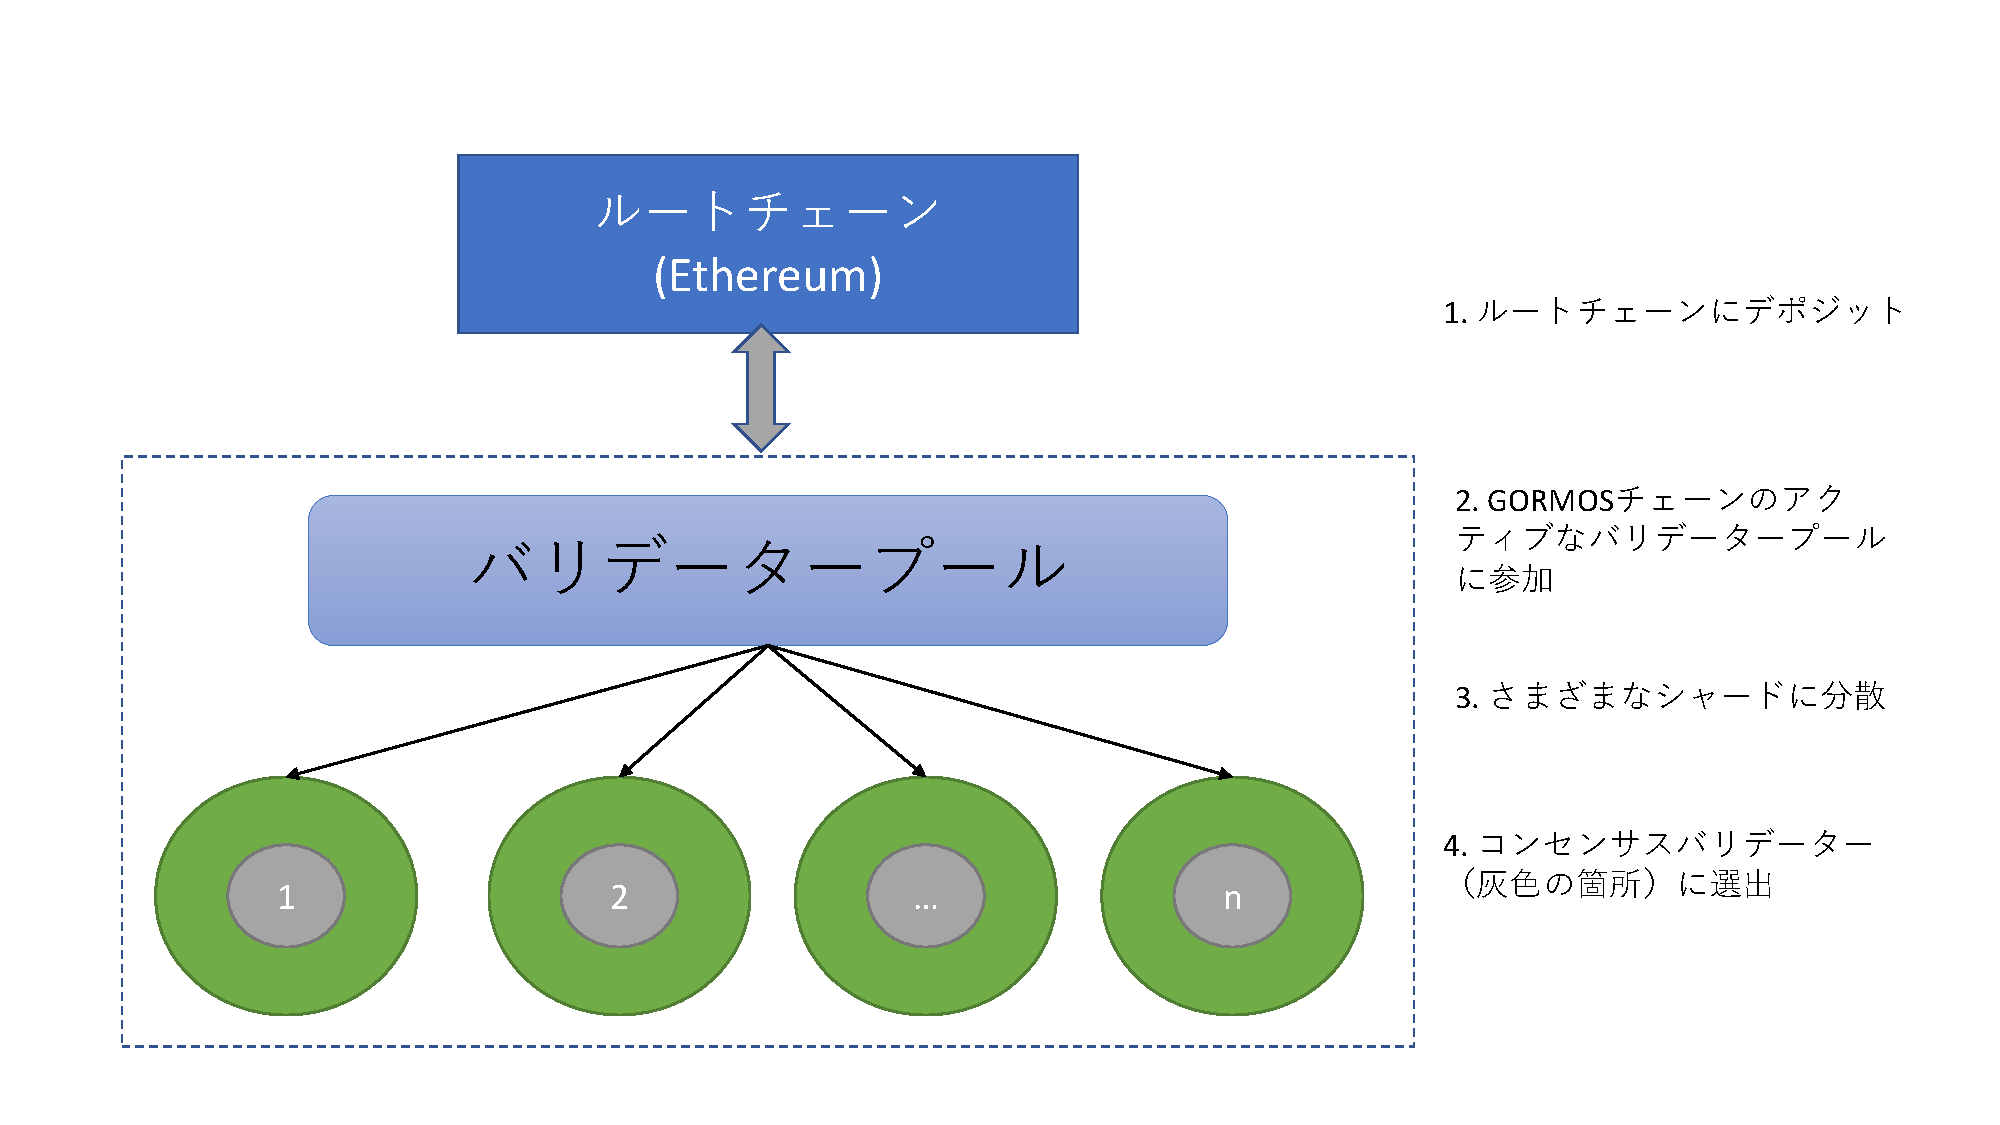
\includegraphics[width=0.8\textwidth]{images/validator}
  \caption{Steps to be validators in \codename}
  \label{fig:validator}
\end{figure}

\subsection{Trade execution and block format}

\textbf{Trade format.} A user in \codename creates a trade order by sending a transaction to the shard. A transaction in a shard would consist of the following information.
\begin{align*}
(\mtt{addr}, \mtt{shard\_id}, \mtt{src\_token\_id}, \mtt{des\_token\_id}, \\ \mtt{order\_type}, \mtt{src\_amount}, \mtt{fee}, \\ \mtt{metadata}, \mtt{nonce}),
\end{align*}

In which
\begin{itemize}
\item $\mtt{addr}$: is the address of the user.
\item $\mtt{shard\_id}$: is the id of the shard that the user is doing the trade with
\item $\mtt{src\_token\_id}$: is the id of the token that the user wants to trade from
\item $\mtt{des\_token\_id}$: is the token that the user wants to trade to
\item $\mtt{order\_type}$: limit orders or market orders, or even a cancel request of an existing order.
\item $\mtt{src\_amount}$: amount of source tokens that the user wants to trade from
\item $\mtt{fee}$: how much fees (in \%) that users wanted to pay (similar to transaction fees)
\item $\mtt{metadata}$: more data on the order. For example, if $\mtt{order\_type}$ is limit order then the users need to include the price, or if $\mtt{order\_type}$ is canceled then the $\mtt{metadata}$ will have $\mtt{order\_id}$, which is a hash of some previous order.
\item $\mtt{nonce}$: similar to transaction’s nonce in Ethereum. This is a counter that represents the number of orders that the user has created so far.
\end{itemize}

\textbf{Block format.} There are two blocks in \codename namely local data blocks and main blocks. A local data block in a shard is comprised of the raw new transaction data, and the data block headers that has the following fields.

\begin{align*}
(\mtt{shard\_id}, \mtt{block\_number}, \mtt{prev\_block\_hash},\\ \mtt{new\_order\_merkle\_root}, \mtt{balance\_merkle\_root}, \mtt{avail\_balance\_merkle\_root},\\ \mtt{open\_order\_MMR\_root}, \mtt{closed\_order\_MMR\_root}, \mtt{cancelled\_order\_MMR\_root},\\ \mtt{timestamp}, \mtt{signatures}),
\end{align*}

in which
$\mtt{shard\_id}$: is the id of the shard that the user is doing the trade with
$\mtt{new\_order\_merkle\_root}$: the Merkle root that commits all new orders in this block
$\mtt{balance\_merkle\_root}$: the Merkle root that commits balances of everyone in the shard after accepting all new orders in this block.
$\mtt{avail\_balance\_merkle\_root}$: the Merkle root that commits available balances of everyone in the shard after accepting all new orders in this block.
$\mtt{open\_order\_MMR\_root}$: the Merkle Mountain Range’s root that commits all open orders in this shard
$\mtt{closed\_order\_MMR\_root}$: the Merkle Mountain Range’s root that commits all closed orders in this shard
$\mtt{cancelled\_order\_MMR\_root}$: the Merkle Mountain Range’s root that commits all cancelled orders in this shard

The main blocks, on the other hand, store all local block headers from local shards and synthesize the results in a single main block header. For example, the block header of the main block can be as follows.

\begin{align*}
(\mtt{block\_number}, \mtt{prev\_block\_hash}, \mtt{new\_local\_headers\_merkle\_root}, \\ \mtt{new\_order\_merkle\_root}, \mtt{balance\_merkle\_root}, \mtt{avail\_balance\_merkle\_root}, \\ \mtt{open\_order\_MMR\_root}, \mtt{closed\_order\_MMR\_root}, \mtt{cancelled\_order\_MMR\_root},\\ \mtt{timestamp}, \mtt{signatures}),
\end{align*}
in which all the new Merkle roots are calculated based on the Merkle roots from the headers of the local blocks.

\textbf{Utilising Merkle Mountain Range.} We leverage Merkle Mountain Range to allow efficient update the Merkle trees for all closed orders, open orders, cancelled orders and so on after every block. \codename utilizes a recently-proposed data structure, called Merkle mountain range (MMR), to allow light clients to efficiently verify any blockchain event with only the latest block.
MMR allows all previous blocks to be efficiently committed to the latest block header in a single hash. One can simply use the original Merkle tree structure to achieve the same goal, however, updating the Merkle trees with new block headers as the leaves is not efficient. One either has to restructure the entire Merkle tree or suffer an ``unbalanced" tree which may yield a proof size of much larger than $\log{n}$ hashes. MMR is a variant of the original Merkle tree that allows a much more efficient update process, thus the overhead for full nodes when processing blocks becomes negligible.

\subsection{Consensus protocol within a shard}\label{shard-consensus}
In Plasma, one can rely on centralized consensus scheme like Proof of Authority without sacrificing security, as suggested in Minimal Viable Plasma~\cite{plasma-mvp} and Plasma Cash~\cite{plasma-cash}. However, due to the need for decentralization to achieve better fault tolerance and censorship resistance, we choose an efficient BFT protocol in each shard to run a reasonably large number of validators. For example, HoneyBadger BFT\cite{honeybadger} which achieves high throughput ($\approx 1.2*10^4\hspace{3pt} tx/s$ with 64 nodes) in an asynchronous network is a good candidate.

\textbf{Practical asynchronous BFT in sporadic layer-2 network}. The validators within a shard shall operate in a different p2p network, separated from the underlying network in the root chain.
% With geographically dispersed nodes in a sporadic WAN setting, this second layer network is more unpredicatable thus leaving candidates whose liveness property relies on partial or weak synchrony assumption less suitable, including likes of PBFT-family\cite{byzantine, zilliqa, tendermint} and more recently proposed Algorand~\cite{algorand}.
Our goal is to allow the shards to propose their new blocks as fast as the network permits, but with an average of 2 second block time. Blocks in different shards are produced in asynchronous manner, i.e. different shards finalize their blocks in different speed, and main shard includes all available local blocks when producing its main blocks. As such, we plan to utilize asynchronous atomic broadcast protocol with optimization proposed by HoneyBadger BFT~\cite{honeybadger}, and threshold public-key encryption to prevent targeted attack and more efficient instantiation of asynchronous common subsets.

% \textbf{Committee rotation in non-deterministic asynchronous protocols}. As deterministic asynchronous agreement is impossible proven by FLP impossibility result \cite{flp-impossibility}, most distributed consensus algorithm either weaken the synchrony assumption or use randomized agreement as work around. In our choice of HoneyBadger BFT, we opt for the latter, which makes validator set rotation harder. It is still an open problem on how to do periodical sortition efficiently and securely, but note that even with a fixed set of priorly known validators, nothing is compromised as far as security and robustness of the system is concerned. Operating in a so-called "permissioned" environment was common argument against HoneyBadger, but such requirement is totally acceptable on Plasma Chain.

\subsection{Fraud proof submission and exit}
We discuss how user can submit fraud proof to root chain, and successfully exit the \codename chain if anything malicious happens. Assuming data availability is upheld by shard inspectors, consider the two possible cases: one is when colluding validators (and corrupted inspectors) within a shard include invalid transactions (i.e. no valid signature, or mismatched input, output amount); the other possibility is an asynchronous network due to either network outrage or deliberate message dropping by adversaries, which stall the shard from making progress.

The user obtains a fraud proof by sending a request to full node, which could be shard inspectors or more conveniently himself if the user runs a full node. In the request the user sent, he/she specifies the specific block that he “agrees” to, meaning any other blocks further down the chain are deemed as invalid. The response from the full node is a Merkle Proof of the user’s balance in the state tree at that particular block height. Put it informally, the user is essentially stating: “I hereby consent to this balance as my latest balance, and I want to exit because either the next block contains illegitimate signatures or it stops working”

In the first scenario, the user submits two Merkle paths to the root chain (Ethereum) \texttt{-{}-} one is the Merkle path of the latest valid balance in the state tree; the other is the path of the invalid state forged by the malicious validators. Since the periodical commit of the plasma main shard, the root chain could verify the Merkle Proof provided, and opens up a challenge period once the proof is valid. During this period, unless the malicious validators could provide a valid transaction with legitimate signature from the user that indicates a state transitions from the former to the latter, the validators will be punished and their deposit forfeited, while users successfully exiting the chain with latest valid balance.

In the second case, it is also doable for each users in that shard to exit one by one, which is quite expensive as they are all on-chain settlements. One could use ``mass withdraw" approach suggested in Plasma to reduce the number of messages on-chain~\cite{plasma}. A good property that \codename offers is that exiting from one shard does not affect the rest of the shards. With damages isolated, \codename's design is more robust.

\subsection{Incentive for validators}
The main incentive for being a validator is getting transaction fees from all processed trades in a shard. This is more obvious for validators that participate in the consensus rounds. We next discuss the incentive for the shard inspectors, who store a full-node data for that shard and monitor if any wrongdoings happen within the shard.

First, shard inspectors are eligible candidates for the next round validators in the same shard, without the entirety of the data, it is impossible to validate the new coming transactions. In addition, only shard inspectors will be selected to participate in the consensus in the shard.

Second, once they spot any wrongdoings, they could submit fraud proofs for users and get rewards from forfeited deposit, and since they are mostly online and monitor the shard more closely than users, it should usually be their chance to catch the potential bad validators. In addition, as inspectors/full-nodes, they also receive smaller fraction of the transactions fee (compared to consensus validators).

\subsection{\codename for other use cases}
\label{sec:others}

We discuss how other applications, apart from decentralized exchanges, can use \codename to allow more transactions to happen on-chain in a scalable and low latency way. As discussed in Section~\ref{sec:intro}, \codename's scalability comes from separating the activities to different shards. As a result, \codename suits better for applications that have separate components, and there are not much interaction between these components. These applications will generate less cross-shard transactions and reduce pressure on the main-shard.
For example, Etheremon is a game that resembles PokemonGO, allowing users to train and grow their ``monsters" and compete with others. The monster can travel to different ``gyms" which belong to different places in the game map. Using \codename, Etheremon can split their map into different local maps corresponding to different shards, each shard represents a geographical region in the game. A shard will manage all monsters and activities within its respective local map. Users can move their monsters to different local maps by sending a transaction to the main shard to indicate the new local map that they want to reside their monsters. As most activities in Etheremon happen within the gyms or when the monsters meet each other in the same location, \codename is arguably the best design to scale up Etheremon without affecting user experience.

Similarly, one can use \codename for other use cases like decentralized Uber,
in which all trips, payments, ratings are recorded on-chain. A \codename-based
Uber can have different shards, each is responsible for a city. The validators
in a shard will verify all transactions in the city and include in the local
blocks. Typically, any application that can be geographically distributed, or
architecturally separated into different components can benefit from
\codename.
